\chapter{Apresentação do Sistema}
\label{cap:exemplos}

% figuras estão no subdiretório "figuras/" dentro deste capítulo
\graphicspath{\currfiledir/figuras/}

%=====================================================
\begin{figure}[!htb]
\centering
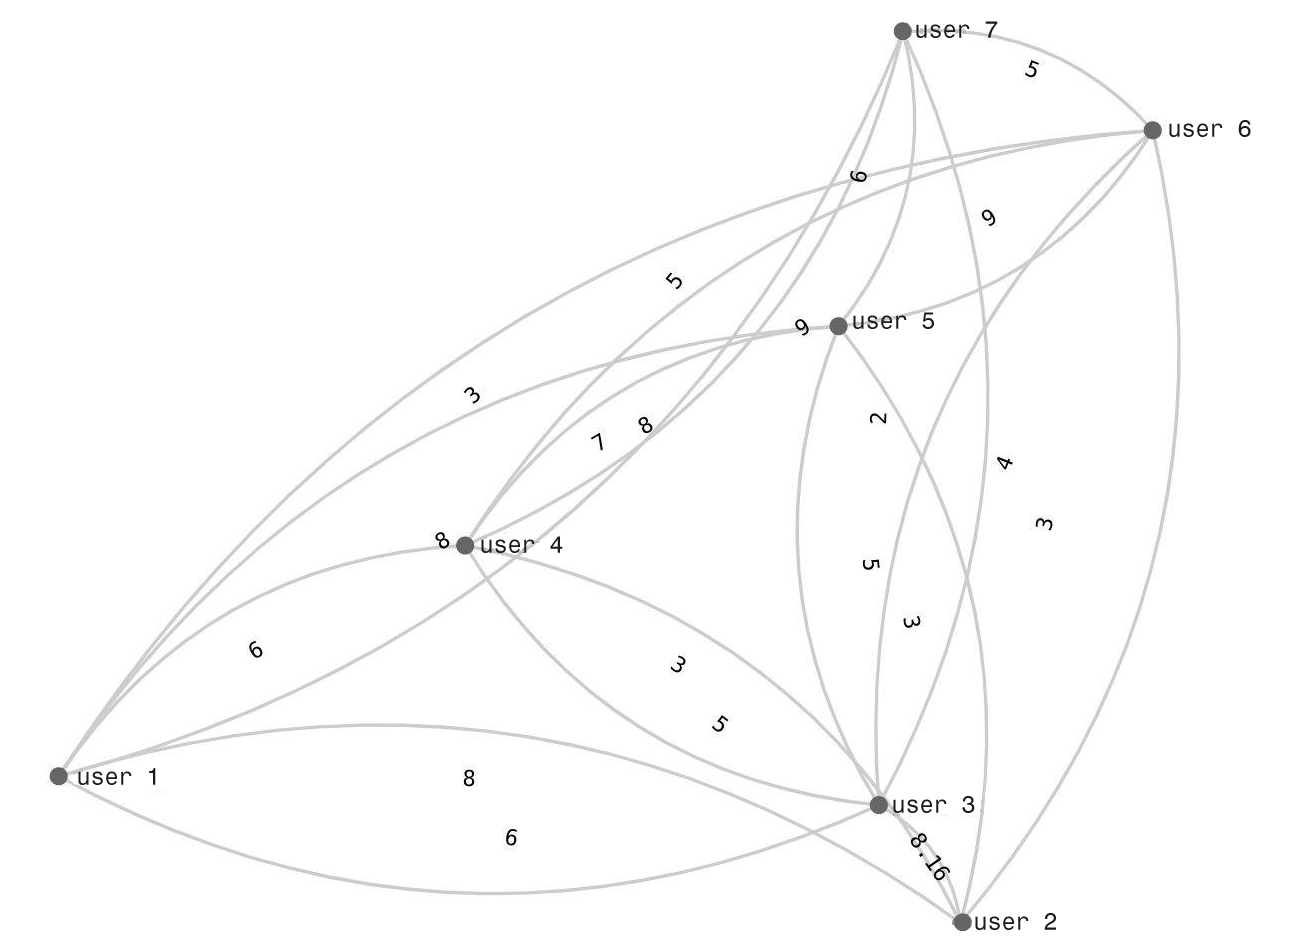
\includegraphics[width=16cm]{grafo.png}
\caption{Grafo representando os usuários do sistema e suas relações. Fonte: os autores.}
\label{fig:grafoproduto}
\end{figure}

O sistema pronto implementou todas as funcionalidades previstas na análise de requisitos. Contou também com a opção de gerar uma imagem do grafo com todos os usuários cadastrados. Na Figura \ref{fig:grafoproduto}, podemos visualizar um grafo gerado pelo software com os usuários registrados até o momento e as respectivas arestas representando o grau de afinidade entre dois nós. A geração desta imagem não é uma funcionalidade do aplicativo, apenas uma ferramenta desenvolvida para ter funcionalidade administrativa e científica.

Na implementação foi aplicada a seguinte função para $k$:

\begin{equation}
k_{ab}=(R_{abA}+R_{baA})-\frac{R_{ab}+R_{ba}}{w}
\label{eq:k8}
\end{equation}

Onde $w$ foi estabelecido como sendo igual a 5 e $x$ igualmente 5.

A apresentação do sistema foi dividida em duas partes com o intuito de acompanhar o caminho do usuário ao utilizar. Dessa maneira as seções são as seguintes:

\begin{itemize}
\item Telas de Perguntas e Respostas
\item Tela do mensageiro instantâneo
\end{itemize}

\section{Perguntas e respostas}
\FloatBarrier

\begin{figure}
\centering
\begin{minipage}{0.45\textwidth}
\centering
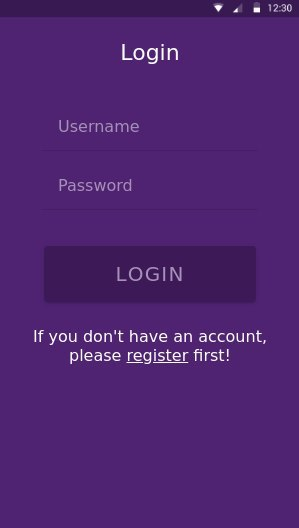
\includegraphics[width=6cm]{telalogin.png}
\caption{Tela de login. Fonte: os autores.}
\label{fig:telalogin}
\end{minipage}\hfill
\begin{minipage}{0.45\textwidth}
\centering
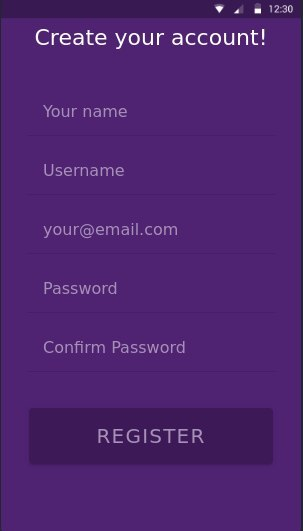
\includegraphics[width=6cm]{telaregister.png}
\caption{Tela de registro. Fonte: os autores.}
\label{fig:telaregister}
\end{minipage}
\end{figure}

A Figura \ref{fig:telalogin} é a tela de login do sistema. As cores a partir daqui seguem o mesmo padrão. Foi escolhida uma cor que pudesse ser afirmada como a representação da identidade do sistema. Assim, a cor é memorável por ser incomum. Tendo em vista que o público esperado para o sistema seja majoritariamente jovem, supõe-se que deve ser bem recebida a excentricidade da cor.

A tela de registro pode ser vista na Figura \ref{fig:telaregister}, segue o mesmo padrão da tela de login, portanto, com a mesma identidade visual.

\begin{figure}
\begin{minipage}{0.45\textwidth}
\centering
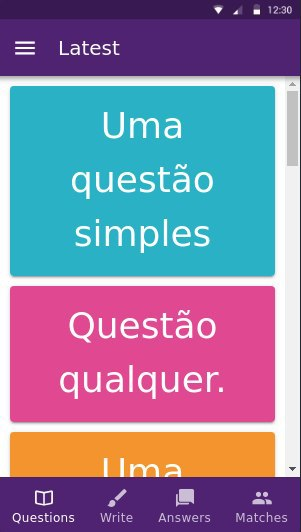
\includegraphics[width=6cm]{telaQuestoes.png}
\caption{Tela de visualização de questões. Fonte: os autores.}
\label{fig:telaQuestoes}
\end{minipage}\hfill
\begin{minipage}{0.45\textwidth}
\centering

\includegraphics[width=6cm]{telaCriarQuest.png}
\caption{Tela de criação de questões. Fonte: os autores.}
\label{fig:telaCriarQuest}
\end{minipage}\hfill
\end{figure}

A tela de visualização de questões pode ser vista na Figura \ref{fig:telaQuestoes}. As cores do balão que contém o texto da pergunta podem ser escolhidas pelo usuário que criou a pergunta. Essas cores foram selecionadas para combinarem integralmente com a cor roxa das barras do aplicativo.

A cor do fundo da questão pode ser escolhida pelo botão no canto inferior direto da tela de criação de questão, como pode ser observado na Figura \ref{fig:telaCriarQuest}. Com um toque no botão as cores mudam cíclicamente.

\begin{figure}
\begin{minipage}{0.45\textwidth}
\centering
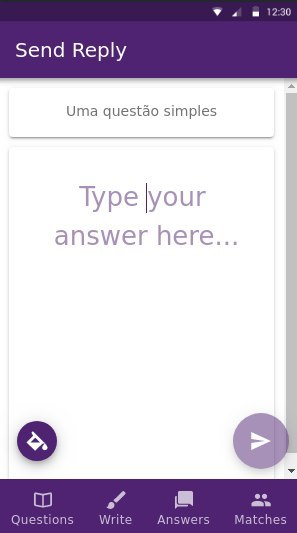
\includegraphics[width=6cm]{telaResponder.png}
\caption{Tela de resposta para questões. Fonte: os autores.}
\label{fig:telaResponder}
\end{minipage}\hfill
\begin{minipage}{0.45\textwidth}
\centering
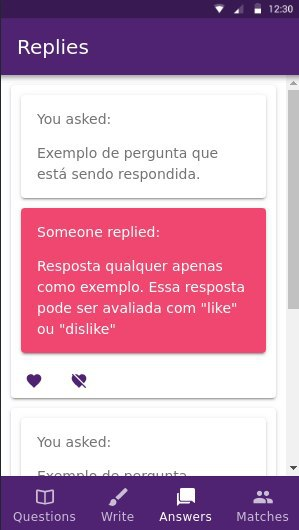
\includegraphics[width=6cm]{telaVerResp.png}
\caption{Tela de visualização de respostas. Fonte: os autores.}
\label{fig:telaVerResp}
\end{minipage}\hfill
\end{figure}

A mesma função de mudar o fundo da tela está presente na tela de criação de respostas, vide Figura \ref{fig:telaResponder}. A cor escolhida para a resposta pode ser visualizada pelo usuário que recebeu a resposta, como podemos observar na Figura \ref{fig:telaVerResp}, que é a tela de visualização de respostas.


%=====================================================

\section{Mensageiro instantâneo}

Depois que os usuários interagem suficientemente o sistema decide criar uma relação entre eles, o contato sugerido aparece disponível no botão \emph{matches}, no canto inferior direito da tela, como podemos observar na Figura \ref{fig:telaContatos}.

A partir desta tela, quando o usuário seleciona um contato é apresentada a tela de conversa, que podemos visualizar na Figura \ref{fig:telaChat}.


\begin{figure}
\begin{minipage}{0.45\textwidth}
\centering
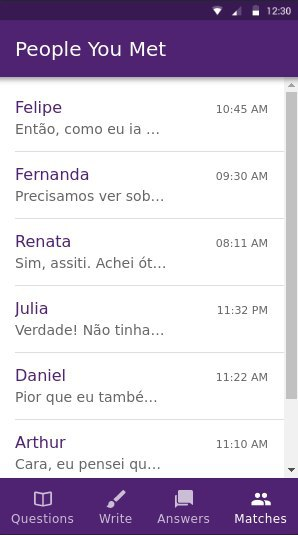
\includegraphics[width=6cm]{telaContatos.png}
\caption{Tela de visualização dos contatos criados. Fonte: os autores.}
\label{fig:telaContatos}
\end{minipage}\hfill
\begin{minipage}{0.45\textwidth}
\centering
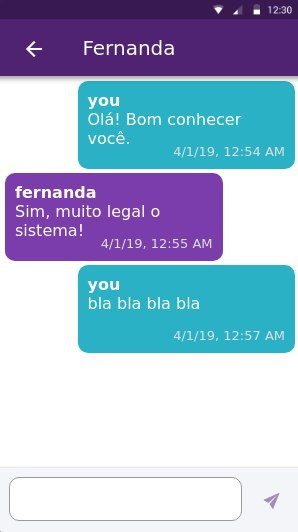
\includegraphics[width=6cm]{telaChat.png}
\caption{Tela de visualização das mensagens recebidas no mensageiro instantâneo. Fonte: os autores.}
\label{fig:telaChat}
\end{minipage}\hfill
\end{figure}

